% Paquets généraux
\documentclass[a4paper,12pt,titlepage]{article}
\usepackage[T1]{fontenc}
\usepackage[utf8]{inputenc}
\usepackage[french]{babel}
\usepackage[gen]{eurosym}
%\usepackage[dvips]{graphicx}
\usepackage{fancyhdr}
\usepackage{pdfpages} 
\usepackage{multido}
\usepackage{hyperref}
%\usepackage{textcomp}
%\usepackage{aeguill}
\usepackage{schemabloc}
\usepackage[bitstream-charter]{mathdesign}
\usepackage{pstricks}
\usepackage{helvet}

\newcommand{\id}{54}
\newcommand{\nom}{Liaisons mécaniques}
\newcommand{\sequence}{04}
\newcommand{\num}{01}
\newcommand{\type}{TP}
\newcommand{\descrip}{Modélisation d'un solide. Comportement des liaisons mécaniques. Modéliser les mécanismes du laboratoire par un schéma cinématique, paramétré.}
\newcommand{\competences}{A3-C4: Analyse d'architecture et de comportement \\ &  Mod1-C1: Isolement d'un solide ou d'un système de solides \\ &  Mod2-C10-1: Modèle de solide indéformable \\ &  Mod2-C11: Modélisation géométrique et cinématique des mouvements entre solides indéformables \\ &  Mod2-C12: Modélisation cinématique des liaisons entre solides \\ &  Mod2-C15: Modélisation des actions mécaniques \\ &  Rés-C6: Utilisation d'un solveur ou d'un logiciel multi physique \\ &  Com1-C1: Différents descripteurs introduits dans le programme \\ &  Com2-C4: Outils de communication}
\newcommand{\nbcomp}{9}
\newcommand{\systemes}{Plateforme Stewart}
\newcommand{\systemessansaccent}{Plateforme Stewart}
\newcommand{\ilot}{2}
\newcommand{\ilotstr}{02}
\newcommand{\dossierilot}{\detokenize{Ilot_02 Plateforme Stewart}}
\newcommand{\imageun}{Plateforme}

\newcommand{\urlsysteme}{\href{https://www.costadoat.fr/systeme/57}{Ressources système}}
\newcommand{\matlabsimscape}{\href{https://github.com/Costadoat/Sciences-Ingenieur/raw/master/Systemes/Plateforme Stewart/Plateforme_Stewart_Simscape.zip}{Modèle Simscape}}
\newcommand{\solidworks}{\href{https://github.com/Costadoat/Sciences-Ingenieur/raw/master/Systemes/Plateforme Stewart/Plateforme_Stewart_Solidworks.zip}{Modèle Solidworks}}
\newcommand{\edrawings}{\href{https://github.com/Costadoat/Sciences-Ingenieur/raw/master/Systemes/Plateforme Stewart/Plateforme_Stewart.EASM}{Modèle eDrawings}}
\newcommand{\test}{Stewart_param1}
\newcommand{\testi}{Stewart_param2}
\newcommand{\testii}{Stewart_param3}
\newcommand{\testiii}{Stewart_param4}
\newcommand{\testiiii}{Stewart_euler}

\newcommand{\auteurun}{Renaud Costadoat}
\newcommand{\institute}{Lycée Dorian}


\usepackage{color}
\usepackage{xcolor}
\usepackage{colortbl}
\usepackage{helvet}
\renewcommand{\familydefault}{\sfdefault}
\usepackage{amsfonts}
\usepackage{amsmath}
%\usepackage{xspace}
\usepackage{varioref}
\usepackage{tabularx}
%\usepackage{floatflt}
\usepackage{graphics}
\usepackage{wrapfig}
\usepackage{textcomp}
\usepackage{tikz}
\usepackage{wrapfig}
\usepackage{gensymb}
\usepackage[european]{circuitikz}
\usetikzlibrary{babel}
\usepackage{ifthen}
\usepackage{cancel}
\usepackage{etoolbox}
\usepackage{multirow}
%\usepackage{boxedminipage}
\definecolor{gris25}{gray}{0.75}
\definecolor{bleu}{RGB}{18,33,98}
\definecolor{bleuf}{RGB}{42,94,171}
\definecolor{bleuc}{RGB}{231,239,247}
\definecolor{rougef}{RGB}{185,18,27}
\definecolor{rougec}{RGB}{255,188,204}%255,230,231
\definecolor{vertf}{RGB}{103,126,82}
\definecolor{vertc}{RGB}{220,255,191}
\definecolor{forestgreen}{rgb}{0.13,0.54,0.13}
\definecolor{blcr}{rgb}{0.59,0.69,0.84}
\definecolor{blfr}{rgb}{0.32,0.51,0.75}
\definecolor{orfr}{rgb}{0.90,0.42,0.15}
\definecolor{orcr}{rgb}{0.90,0.65,0.50}
\definecolor{orangef}{rgb}{0.659,0.269,0.072}
\definecolor{orange}{rgb}{0.58,0.35,0.063}
\definecolor{orangec}{rgb}{0.43,0.32,0.25}
\definecolor{rcorrect}{rgb}{0.6,0,0}
\definecolor{sequence}{rgb}{0.75,0.75,0.75}
\definecolor{competences}{rgb}{0.61,0.73,0.35}
\definecolor{grisf}{HTML}{222222}
\definecolor{grisc}{HTML}{636363}
\definecolor{normal}{HTML}{4087c4}
\definecolor{info}{HTML}{5bc0de}
\definecolor{success}{RGB}{92,184,92}
\definecolor{warning}{RGB}{240,173,78}
\definecolor{danger}{RGB}{217,83,79}
\hypersetup{                    % parametrage des hyperliens
    colorlinks=true,                % colorise les liens
    breaklinks=true,                % permet les retours à la ligne pour les liens trop longs
    urlcolor= blfr,                 % couleur des hyperliens
    linkcolor= orange,                % couleur des liens internes aux documents (index, figures, tableaux, equations,...)
    citecolor= forestgreen                % couleur des liens vers les references bibliographiques
    }

% Mise en page
\pagestyle{fancy}

\setlength{\hoffset}{-18pt}

\setlength{\oddsidemargin}{0pt} 	% Marge gauche sur pages impaire2s
\setlength{\evensidemargin}{0pt} 	% Marge gauche sur pages paires
\setlength{\marginparwidth}{00pt} 	% Largeur de note dans la marge
\setlength{\headwidth}{481pt} 	 	% Largeur de la zone de tête (17cm)
\setlength{\textwidth}{481pt} 	 	% Largeu\textbf{r de la zone de texte (17cm)
\setlength{\voffset}{-18pt} 		% Bon pour DOS
\setlength{\marginparsep}{7pt}	 	% Séparation de la marge
\setlength{\topmargin}{-30pt} 		% Pas de marge en haut
\setlength{\headheight}{55pt} 		% Haut de page
\setlength{\headsep}{20pt} 		% Entre le haut de page et le texte
\setlength{\footskip}{30pt} 		% Bas de\textbf{ page + séparation
\setlength{\textheight}{700pt} 		% Hauteur de l'icone zone de texte (25cm)
\setlength\fboxrule{1 pt}
\renewcommand{\baselinestretch}{1}
\setcounter{tocdepth}{1}
\newcommand{\cadre}[2]
{\fbox{
  \begin{minipage}{#1\linewidth}
   \begin{center}
    #2\\
   \end{center}
  \end{minipage}
 }
}

\newcommand{\reponse}[1][4]
{
\multido{}{#1}
{\begin{center}\makebox[0.9\linewidth]{}  \\
\begin{center}\makebox[0.9\linewidth]{\dotfill} \\ \end{center}
}}

\newcommand{\titre}[1]
{\begin{center}
\cadre{0.8}{\huge #1} 
\end{center}
}


% En tête et pied de page
\lhead{\nom}
\rhead{
\includegraphics[width=2cm]{../../img/logo}}
\lfoot{Renaud Costadoat}
\cfoot{Page \thepage}

\fancypagestyle{correction}{%
  \fancyhf{}
  \lhead{\colorbox{danger}{\begin{minipage}{0.65\paperwidth} \textcolor{white}{\textbf{Correction}} \end{minipage}} }
  \rhead{
\includegraphics[width=2cm]{../../img/logo}}
  \lfoot{Renaud Costadoat}
  \rfoot{\colorbox{danger}{\begin{minipage}{0.6\paperwidth} \begin{flushright}\textcolor{white}{\textbf{Correction}}\end{flushright} \end{minipage}} }}

\renewcommand{\footrulewidth}{0.4pt}

\usepackage{eso-pic}
\newcommand{\BackgroundPic}{%
\put(0,0){%
\parbox[b][\paperheight]{\paperwidth}{%
\vfill
\begin{center}
\hspace{0.5cm}\vspace{0.5cm}
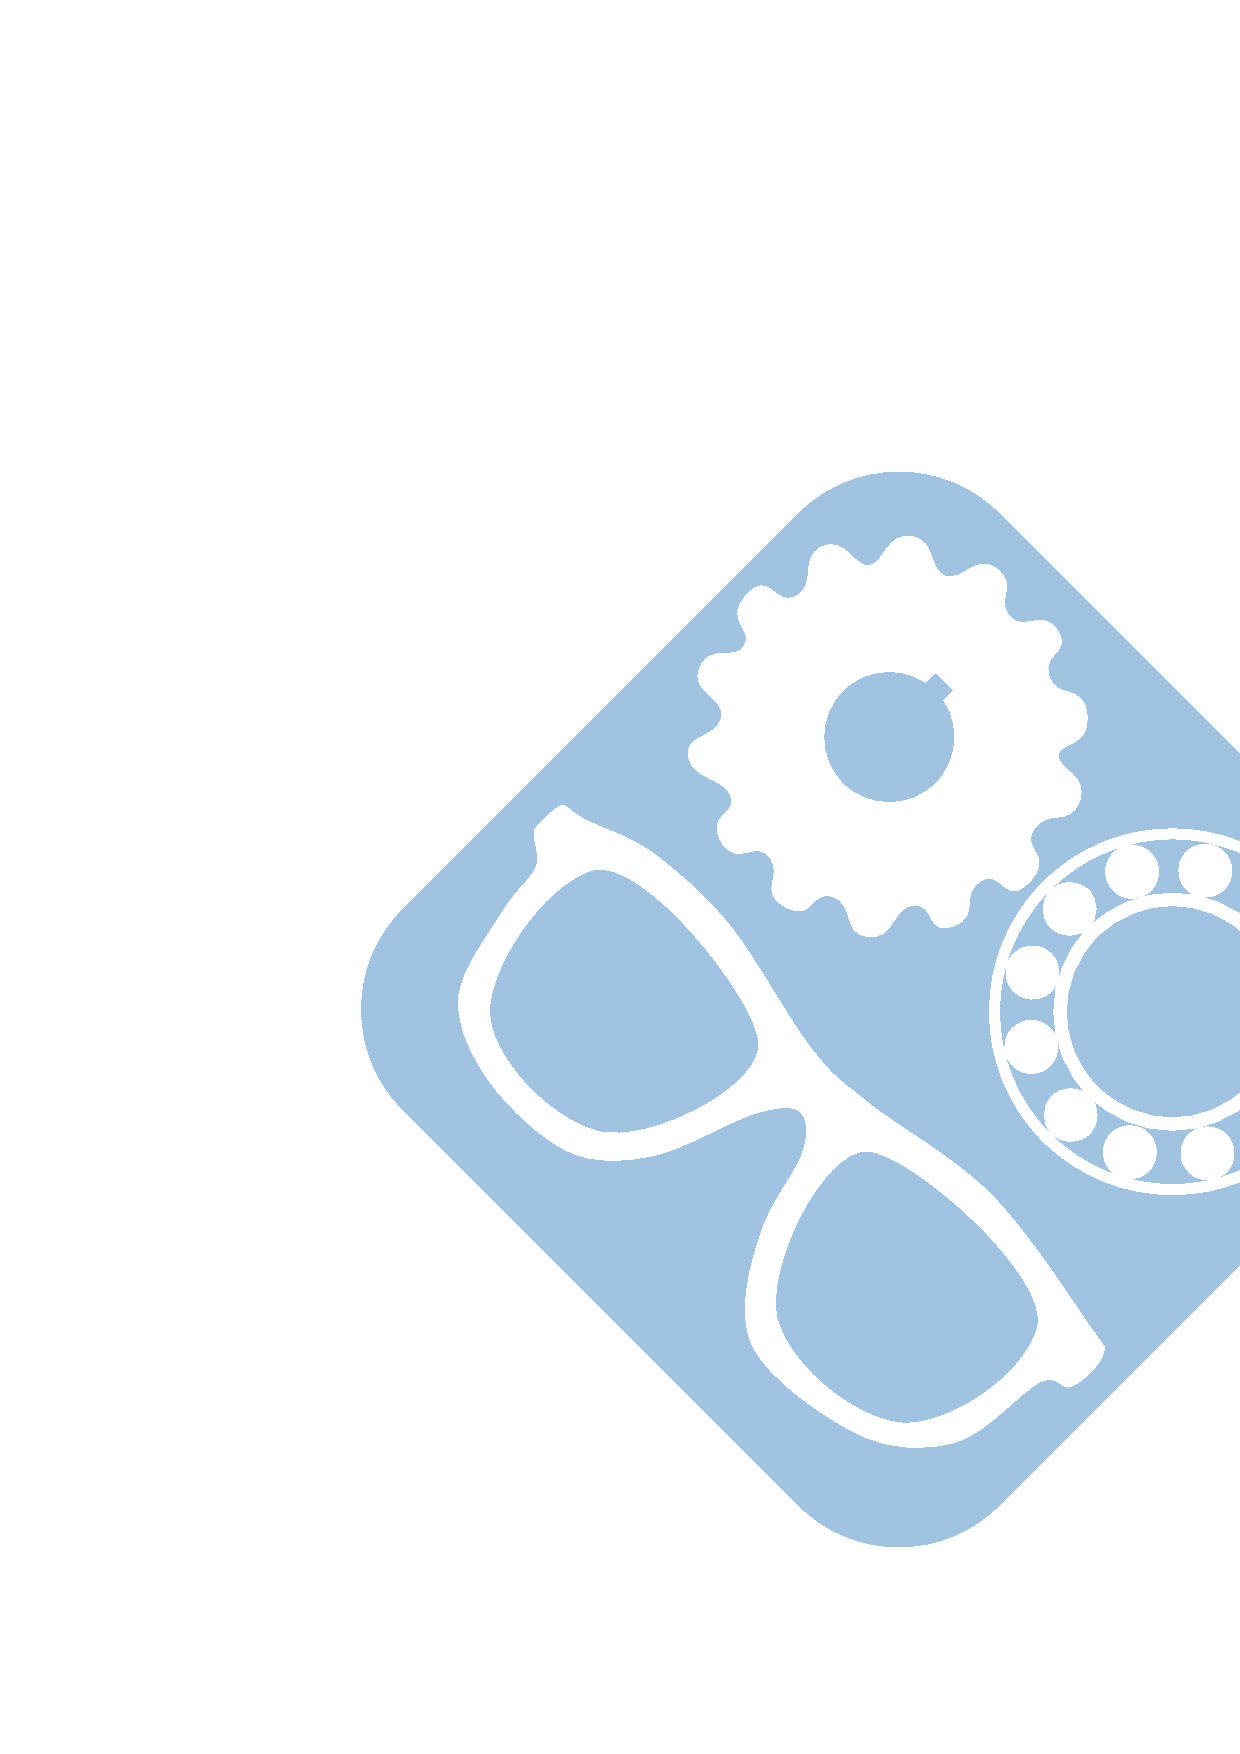
\includegraphics[width=\paperwidth,height=\paperheight,%
keepaspectratio]{../../img/fond3}%
\end{center}
\vfill
}}}

\newcommand{\BackgroundPicdeux}{%
\put(25,-30){%
\parbox[b][\paperheight]{\paperwidth}{%
\vfill
\begin{center}
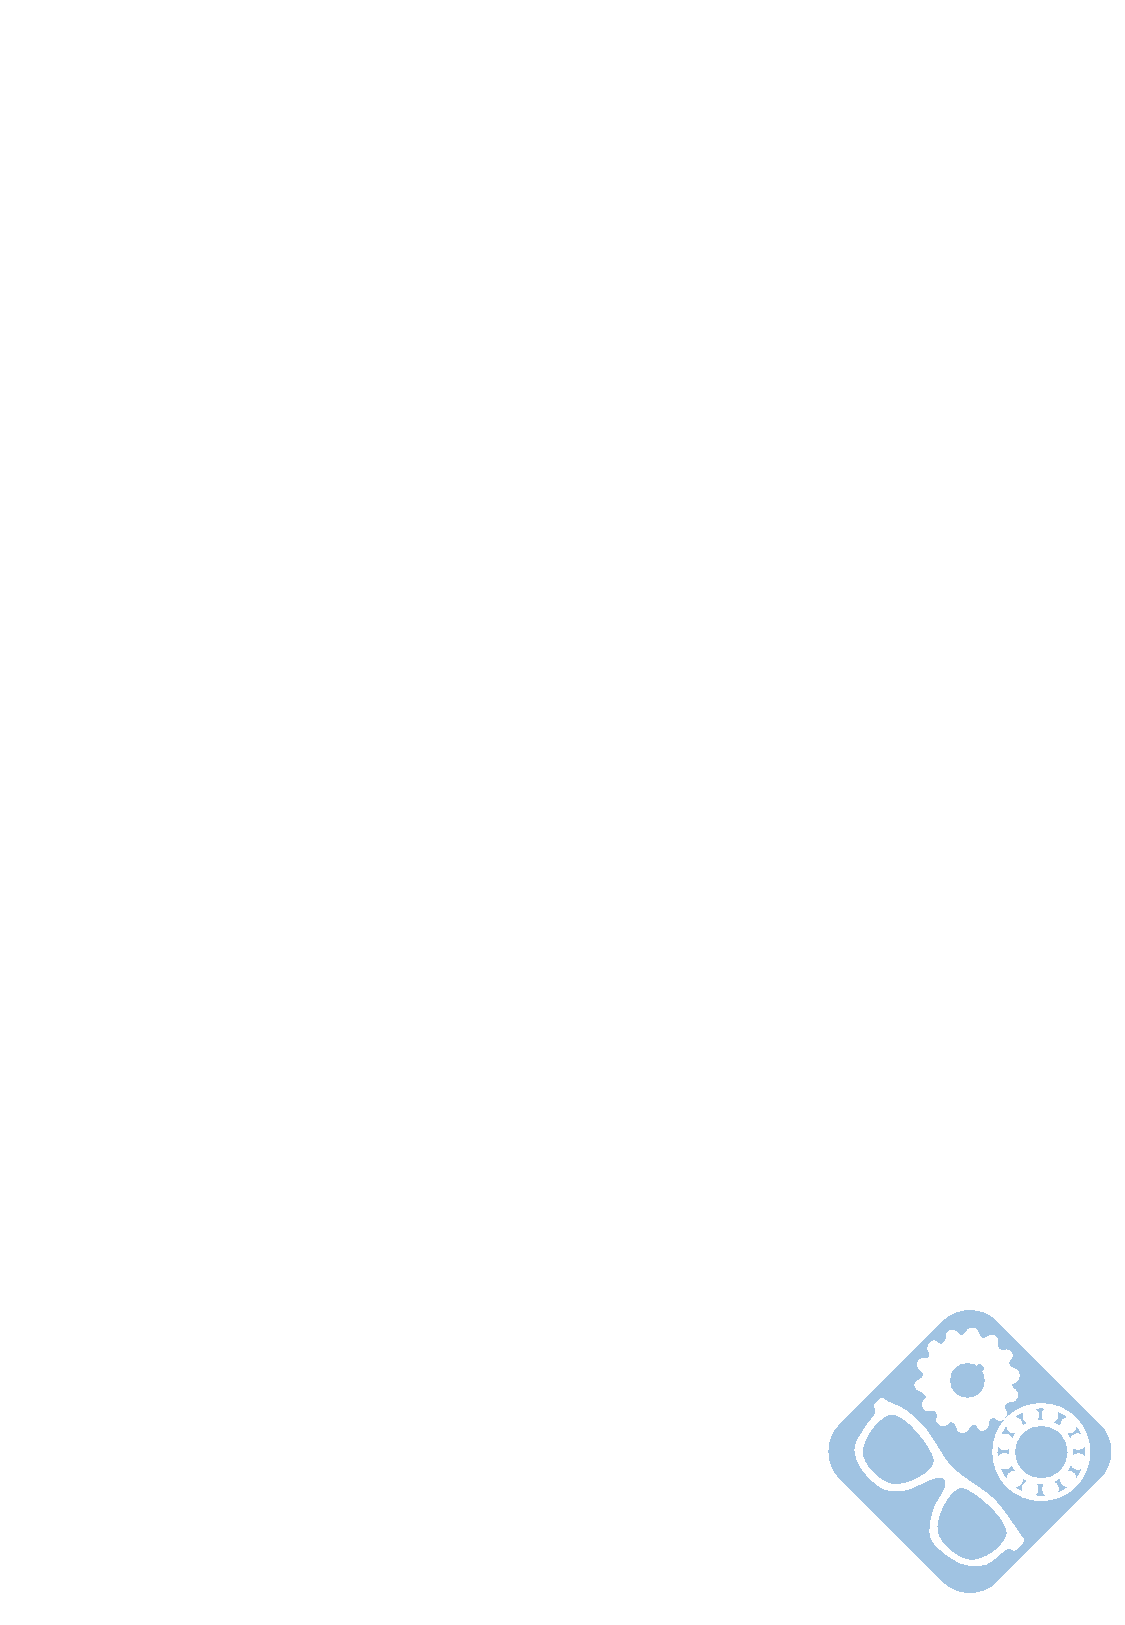
\includegraphics[width=\paperwidth,height=\paperheight,%
keepaspectratio]{../../img/fond4}%
\end{center}
\vfill
}}}

\begin{document}

\AddToShipoutPicture{\BackgroundPicdeux}

\pagestyle{fancy}

\section{Système E.P.A.S.}

\subsection{Présentation}

\begin{figure}[htbp]
\begin{minipage}[c]{.55\linewidth}
Une E.P.A.S. est une Echelle Pivotante Automatique à commande Séquentielle. Ce système est monté sur le châssis d'un camion de pompiers et permet de déplacer une plate forme pouvant recevoir deux personnes et un brancard le plus rapidement possible et en toute sécurité.
\end{minipage}
\hfill
\begin{minipage}[c]{.40\linewidth}
\begin{center}
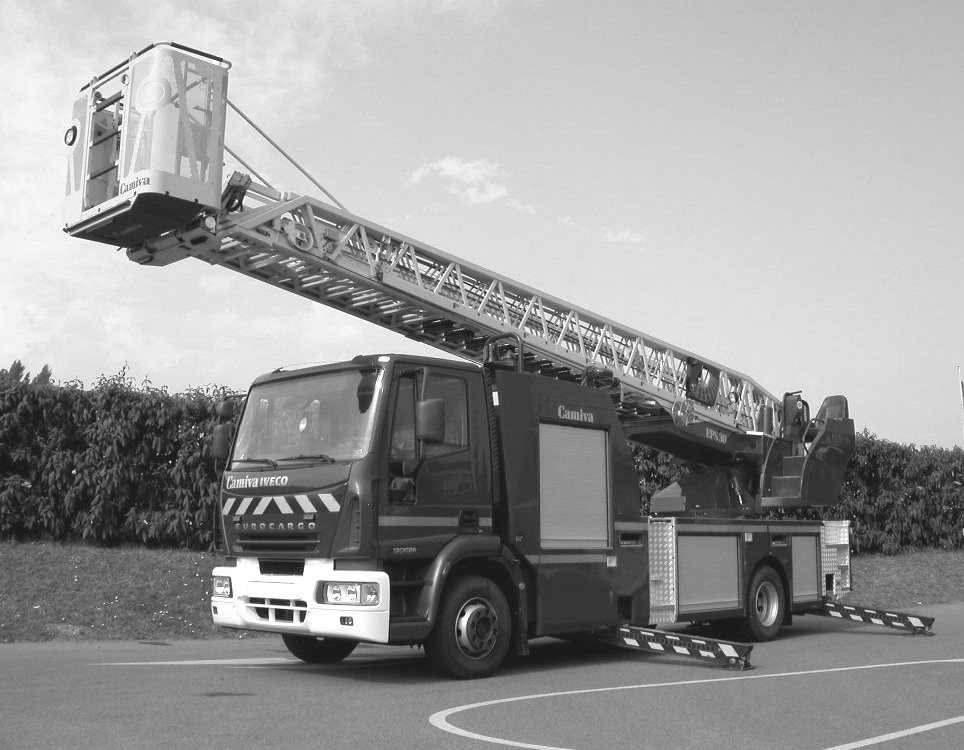
\includegraphics[width=0.8\linewidth]{img/photo_camion.jpg}
\caption{Système E.P.A.S.}
\label{fig:image1}
\end{center}
\end{minipage}
\end{figure}

La figure \ref{fig:image2} présente une vue de côté du camion, celle-ci permet la modélisation géométrique du système.

Les données géométriques sont les suivantes:
\begin{itemize}
 \item la longueur $AC=l_{AC}$,
 \item la longueur $O_0A=l_{O_0A}$,
 \item la longueur $O_0B=l_{O_0B}$,
 \item la longueur $BC=l$.
\end{itemize}

Le paramètre $l$ est variable et correspond à la longueur du vérin.

\begin{figure}[htbp]
\begin{center}
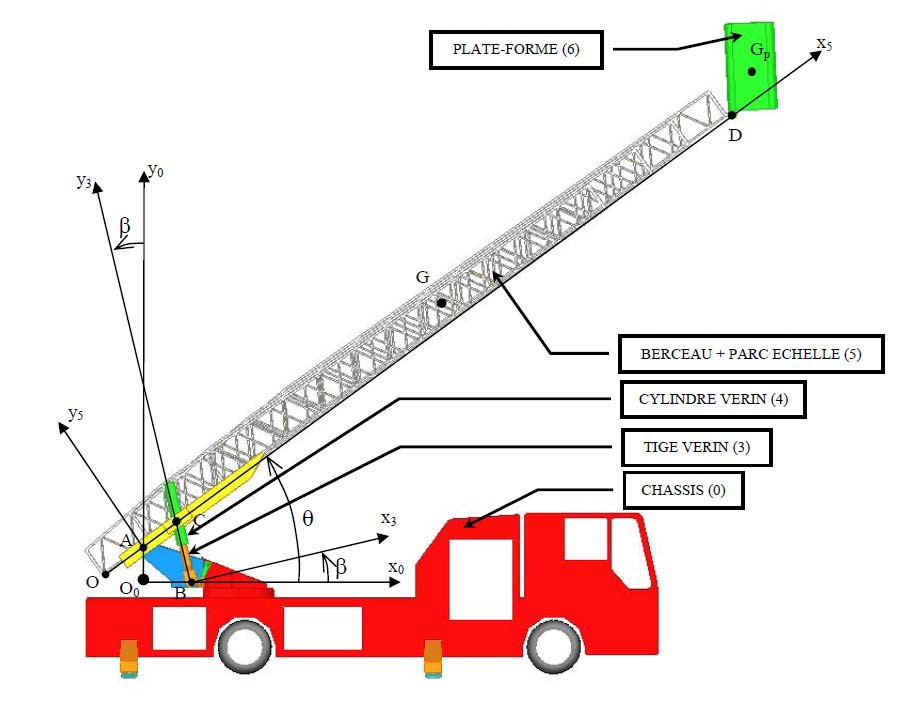
\includegraphics[width=0.6\linewidth]{img/camion.jpg}
\caption{Schéma paramétré du camion}
\label{fig:image2}
\end{center}
\end{figure}

L'exercice porte sur la chaîne de fermeture géométrique suivante:

$\overrightarrow{O_0A}+\overrightarrow{AC}+\overrightarrow{CB}+\overrightarrow{BO_0}=\overrightarrow{0}$

\paragraph{Question 1:}

Écrire les vecteurs:
\begin{itemize}
 \item $\overrightarrow{O_0A}$ dans le repère ($\overrightarrow{x_0}$,$\overrightarrow{y_0}$,$\overrightarrow{z_0}$),
 \item $\overrightarrow{AC}$ dans le repère ($\overrightarrow{x_5}$,$\overrightarrow{y_5}$,$\overrightarrow{z_5}$),
 \item $\overrightarrow{CB}$ dans le repère ($\overrightarrow{x_3}$,$\overrightarrow{y_3}$,$\overrightarrow{z_3}$),
 \item $\overrightarrow{BO_0}$ dans le repère ($\overrightarrow{x_0}$,$\overrightarrow{y_0}$,$\overrightarrow{z_0}$).
\end{itemize}

\paragraph{Question 2:}

Proposer les figures de changement de repères pour passer:
\begin{itemize}
 \item du repère ($\overrightarrow{x_3}$,$\overrightarrow{y_3}$,$\overrightarrow{z_3}$) dans le repère ($\overrightarrow{x_0}$,$\overrightarrow{y_0}$,$\overrightarrow{z_0}$),
 \item du repère ($\overrightarrow{x_5}$,$\overrightarrow{y_5}$,$\overrightarrow{z_5}$) dans le repère ($\overrightarrow{x_0}$,$\overrightarrow{y_0}$,$\overrightarrow{z_0}$).
\end{itemize}

\paragraph{Question 3:}

Écrire les vecteurs:
\begin{itemize}
 \item $\overrightarrow{O_0A}$ dans le repère ($\overrightarrow{x_0}$,$\overrightarrow{y_0}$,$\overrightarrow{z_0}$),
 \item $\overrightarrow{AC}$ dans le repère ($\overrightarrow{x_0}$,$\overrightarrow{y_0}$,$\overrightarrow{z_0}$),
 \item $\overrightarrow{CB}$ dans le repère ($\overrightarrow{x_0}$,$\overrightarrow{y_0}$,$\overrightarrow{z_0}$),
 \item $\overrightarrow{BO_0}$ dans le repère ($\overrightarrow{x_0}$,$\overrightarrow{y_0}$,$\overrightarrow{z_0}$).
\end{itemize}

\paragraph{Question 4:}

Projeter les composantes de la chaîne de fermeture géométrique suivante: $\overrightarrow{O_0A}+\overrightarrow{AC}+\overrightarrow{CB}+\overrightarrow{BO_0}=\overrightarrow{0}$ sur les trois vecteurs de la base: $\overrightarrow{x_0}$, $\overrightarrow{y_0}$ et $\overrightarrow{z_0}$ .

~\

En déduire les relations scalaires qui existent sur ce mécanisme et écrire:
\begin{itemize}
 \item la longueur $l$ du vérin en fonction des autres paramètres du système et de l'angle $\theta$,
 \item l'angle $\beta$ du vérin en fonction des autres paramètres du système et de l'angle $\theta$.
\end{itemize}

\newpage

\section{Pèse lettre}

Le système pèse lettre est un système qui permet de peser le courrier afin de déterminer l'affranchissement nécessaire à son envoie. Les figures \ref{fig:image3} et \ref{fig:image4} présentent des vues d'un de ces mécanismes.

\begin{figure}[htbp]
\begin{minipage}[c]{.48\linewidth}
\begin{center}
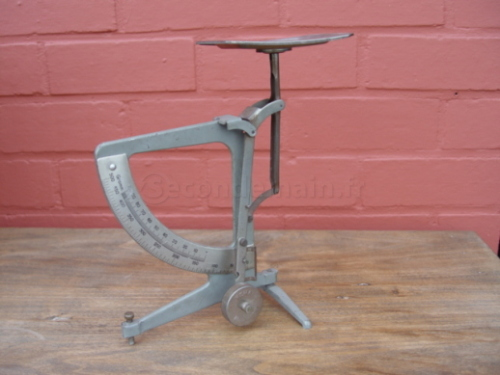
\includegraphics[width=\linewidth]{img/pl_face.jpg}
\caption{Pèse lettre}
\label{fig:image3}
\end{center}
\end{minipage}
\hfill
\begin{minipage}[c]{.48\linewidth}
\begin{center}
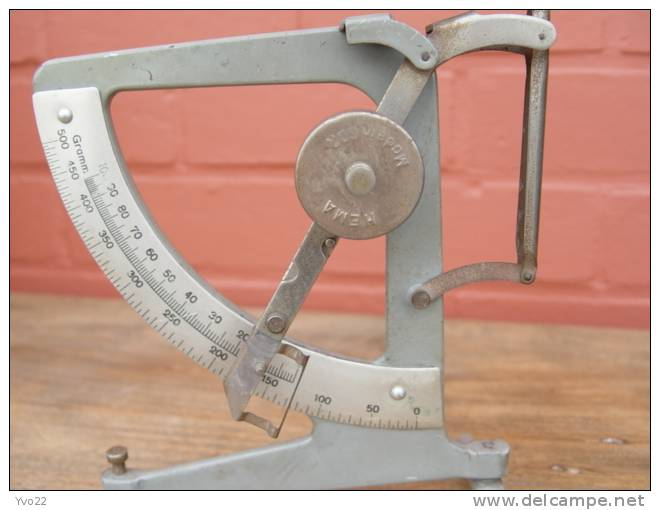
\includegraphics[width=\linewidth]{img/pl_zoom.jpg}
\caption{Zoom sur le pèse lettre}
\label{fig:image4}
\end{center}
\end{minipage}
\end{figure}

\begin{figure}[htbp]
\begin{minipage}[c]{.4\linewidth}
Le mécanisme de transformation de mouvement est présenté à la figure \ref{fig:image5}, il montre comment le mouvement de translation imputé par le poids de l'enveloppe se transforme en rotation de l'aiguille. Le déplacement de la masse sur l'aiguille permet de passer de la pesée d'enveloppes à celle de colis.
\end{minipage}
\hfill
\begin{minipage}[c]{.55\linewidth}
\begin{center}
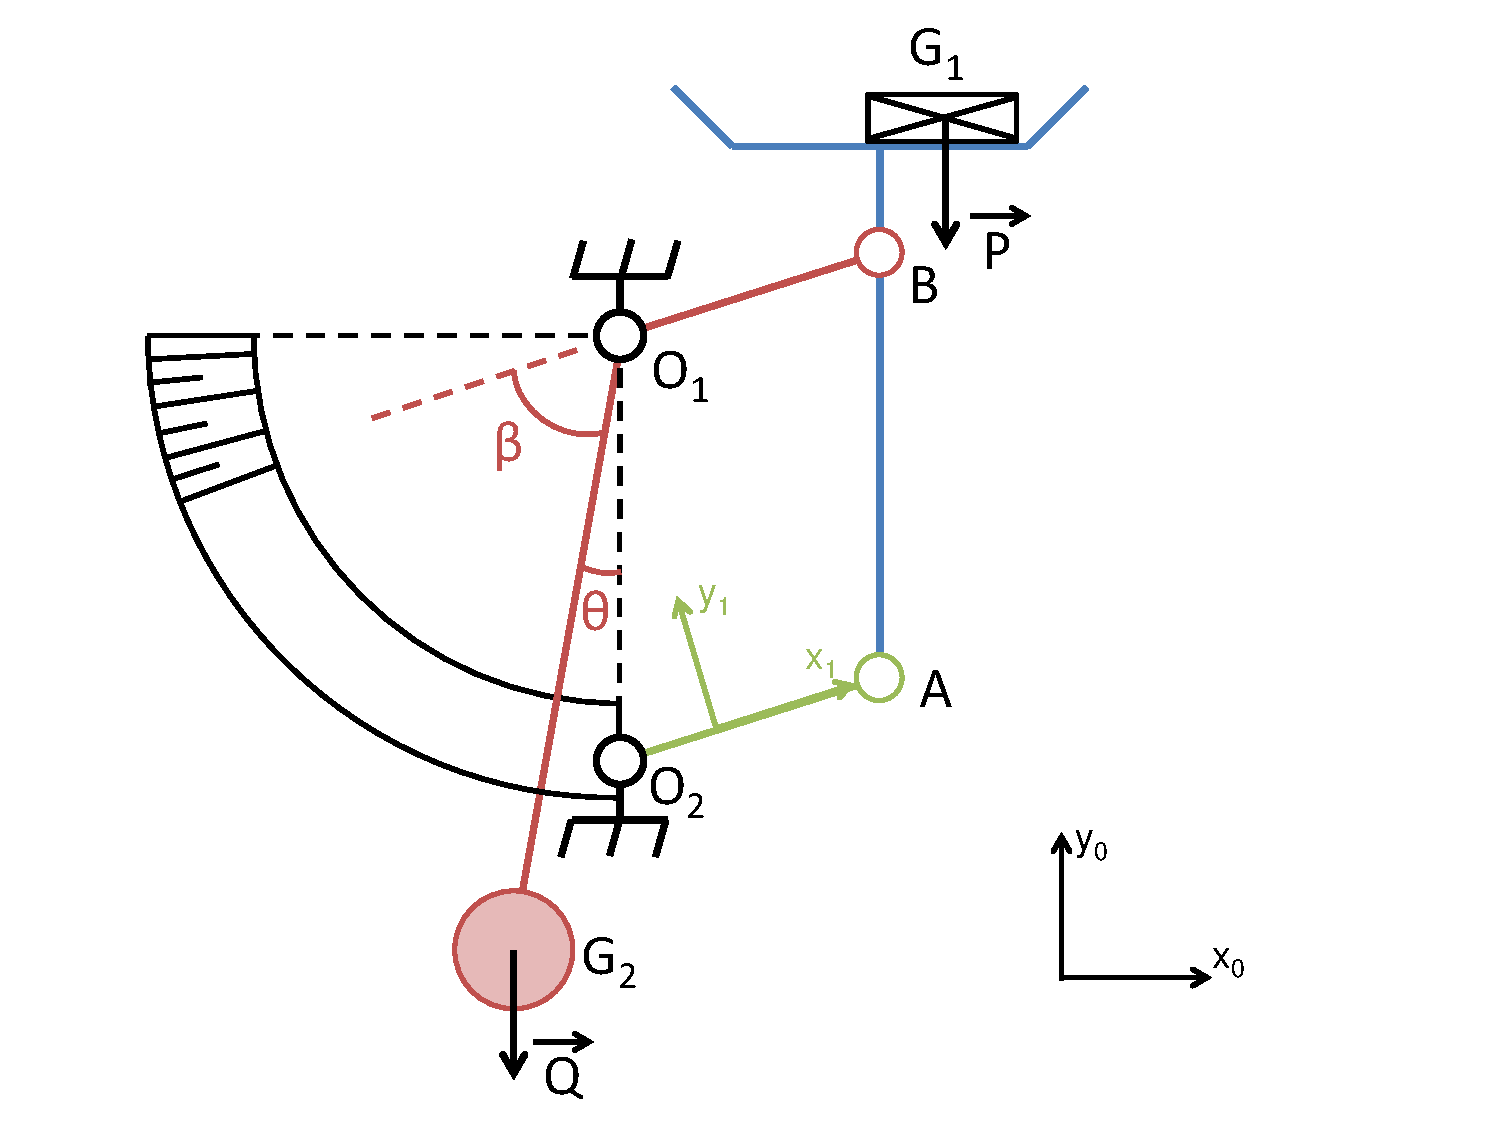
\includegraphics[width=1\linewidth]{img/pl_cin.pdf}
\caption{Schéma cinématique}
\label{fig:image5}
\end{center}
\end{minipage}
\end{figure}

Les données géométriques sont les suivantes:
\begin{itemize}
 \item la longueur $O_1O_2=AB=l_{1}$,
 \item la longueur $O_1B=O_2A=l_{2}$,
 \item la longueur $O_1G_2=l_{3}$.
\end{itemize}

~\

L'exercice porte sur la chaîne de fermeture géométrique suivante:

$\overrightarrow{O_1O_2}+\overrightarrow{O_2A}+\overrightarrow{AB}+\overrightarrow{BO_1}=\overrightarrow{0}$

\paragraph{Question 1:}

Écrire les vecteurs:
\begin{itemize}
 \item $\overrightarrow{O_1O_2}$ dans le repère ($\overrightarrow{x_0}$,$\overrightarrow{y_0}$,$\overrightarrow{z_0}$),
 \item $\overrightarrow{O_2A}$ dans le repère ($\overrightarrow{x_1}$,$\overrightarrow{y_1}$,$\overrightarrow{z_1}$),
 \item $\overrightarrow{AB}$ dans le repère ($\overrightarrow{x_0}$,$\overrightarrow{y_0}$,$\overrightarrow{z_0}$),
 \item $\overrightarrow{BO_1}$ dans le repère ($\overrightarrow{x_1}$,$\overrightarrow{y_1}$,$\overrightarrow{z_1}$).
\end{itemize}

\paragraph{Question 2:}

Proposer les figures de changement de repères pour passer:
\begin{itemize}
 \item du repère ($\overrightarrow{x_1}$,$\overrightarrow{y_1}$,$\overrightarrow{z_1}$) dans le repère ($\overrightarrow{x_0}$,$\overrightarrow{y_0}$,$\overrightarrow{z_0}$).
\end{itemize}

\paragraph{Question 3:}

Écrire les vecteurs:
\begin{itemize}
 \item $\overrightarrow{O_1O_2}$ dans le repère ($\overrightarrow{x_0}$,$\overrightarrow{y_0}$,$\overrightarrow{z_0}$),
 \item $\overrightarrow{O_2A}$ dans le repère ($\overrightarrow{x_0}$,$\overrightarrow{y_0}$,$\overrightarrow{z_0}$),
 \item $\overrightarrow{AB}$ dans le repère ($\overrightarrow{x_0}$,$\overrightarrow{y_0}$,$\overrightarrow{z_0}$),
 \item $\overrightarrow{BO_1}$ dans le repère ($\overrightarrow{x_0}$,$\overrightarrow{y_0}$,$\overrightarrow{z_0}$).
\end{itemize}

\paragraph{Question 4:}

Projeter les composantes de la chaîne de fermeture géométrique suivante: $\overrightarrow{O_1O_2}+\overrightarrow{O_2A}+\overrightarrow{AB}+\overrightarrow{BO_1}=\overrightarrow{0}$ sur les trois vecteurs de la base: $\overrightarrow{x_0}$, $\overrightarrow{y_0}$ et $\overrightarrow{z_0}$. Que pensez-vous du résultat ?

~\

En déduire les relations scalaires qui existent sur ce mécanisme et écrire quel serait le déplacement vertical du point B qui permettrait de faire passer l'aiguille de l'angle $\theta=0$ \textdegree à $\theta=-90$ \textdegree afin de déterminer l'amplitude du déplacement de la mesure.

\newpage

\section{Pince Schrader}

La pince Schrader est une pince utilisée pour la préhension d'objet dans les systèmes automatisée. Elle permet à partir du déplacement d'un vérin de fermer ou d'ouvrir ses doigts afin de pouvoir saisir un objet.

\begin{figure}[htbp]
\begin{minipage}[c]{.4\linewidth}
\begin{center}
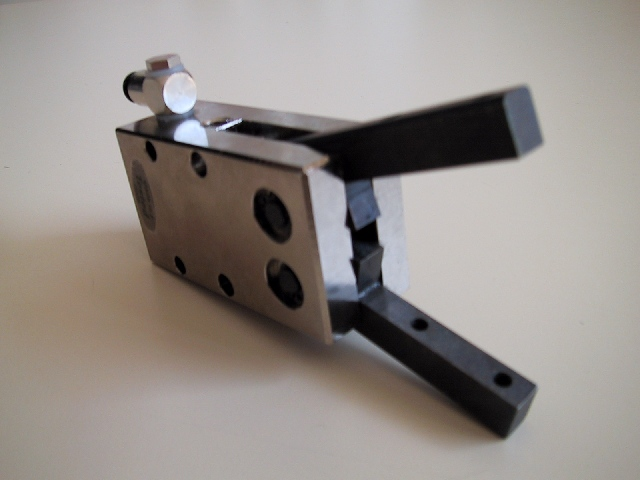
\includegraphics[width=\linewidth]{img/pince_schrader.jpg}
\caption{Pince Schrader}
\label{fig:image6}
\end{center}
\end{minipage}
\hfill
\begin{minipage}[c]{.55\linewidth}
\begin{center}
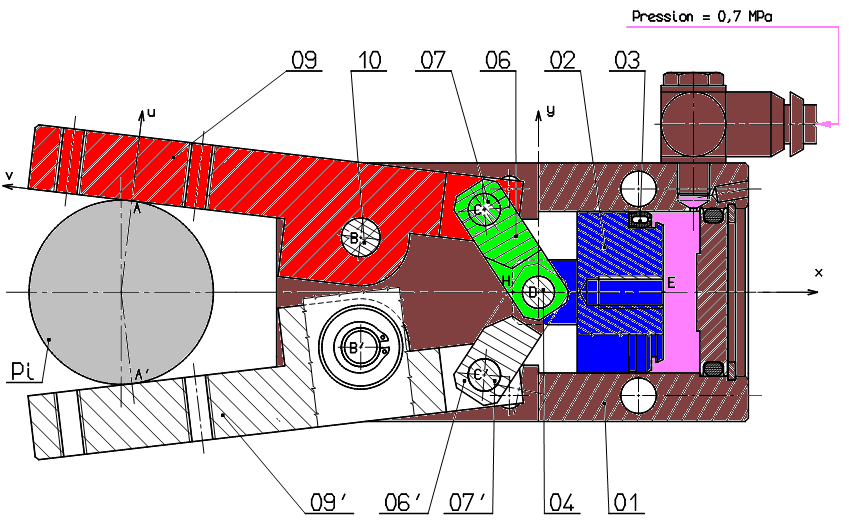
\includegraphics[width=\linewidth]{img/ps_plan.png}
\caption{Plan de la pince}
\label{fig:image7}
\end{center}
\end{minipage}
\end{figure}

\begin{figure}[htbp]
\begin{minipage}[c]{.4\linewidth}
Le schéma cinématique construit à partir du plan de la figure \ref{fig:image7} est présenté à la figure \ref{fig:image8}, il permet l'étude géométrique suivante. Les pièces en pointillés ne sont pas étudiées dans cet exercice.
\end{minipage}
\hfill
\begin{minipage}[c]{.55\linewidth}
\begin{center}
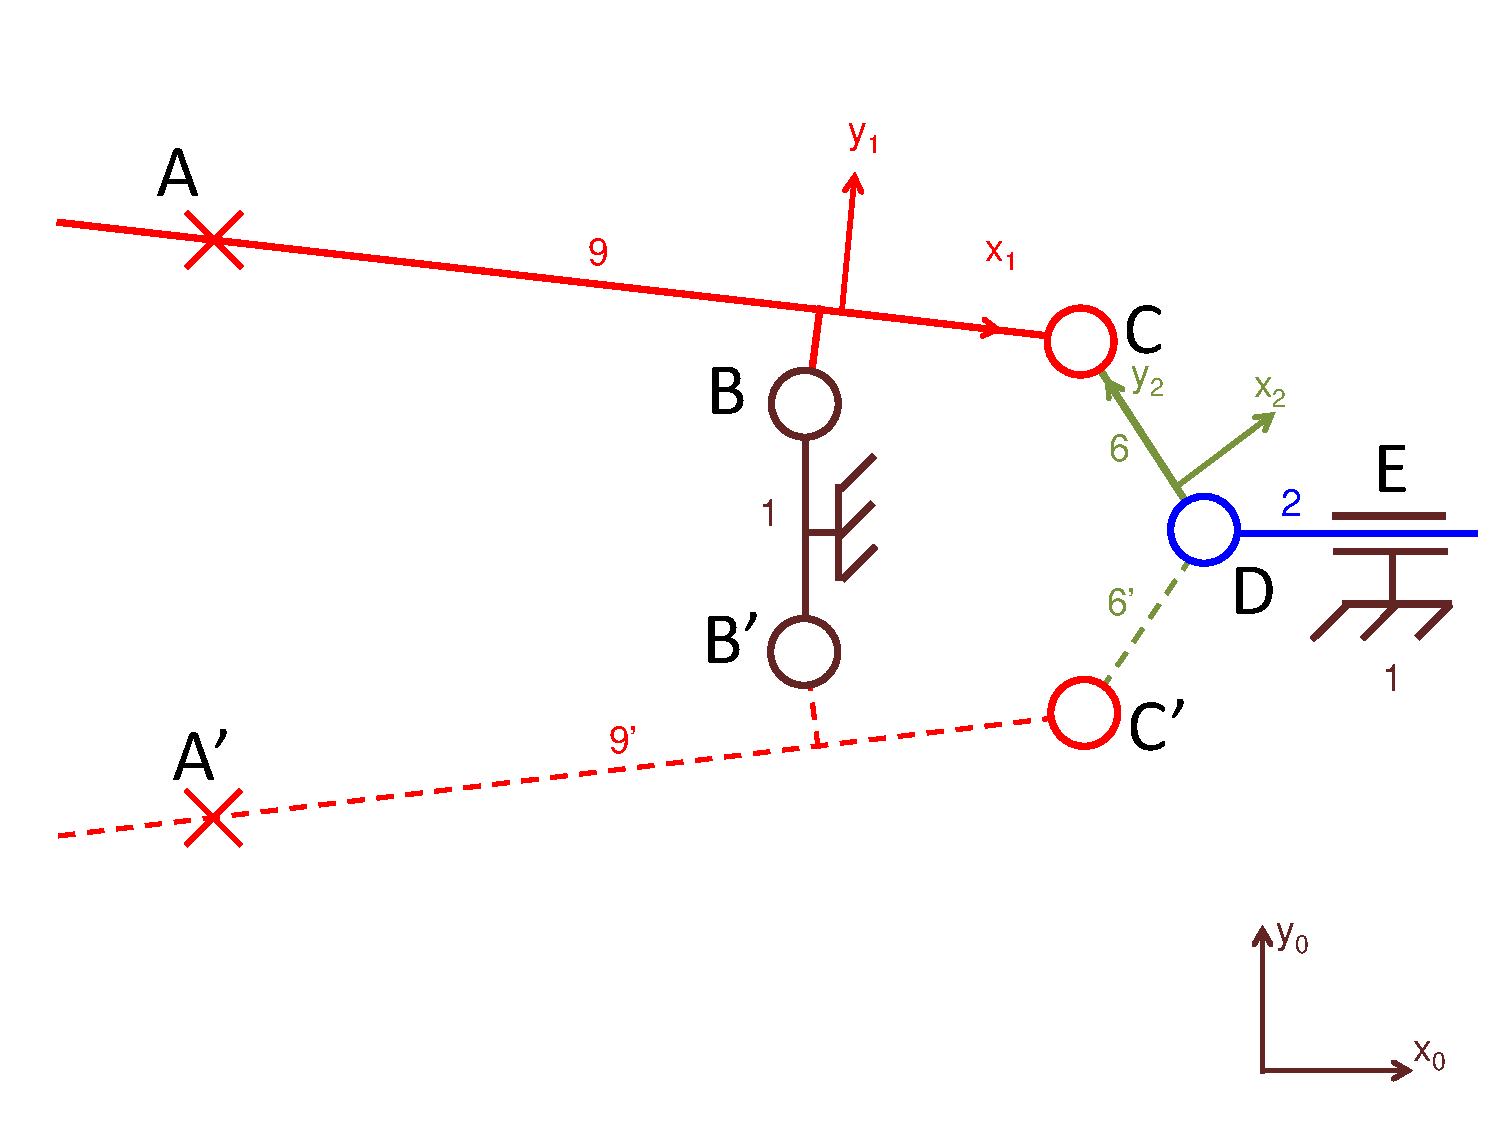
\includegraphics[width=1\linewidth]{img/ps_cin.pdf}
\caption{Schéma cinématique}
\label{fig:image8}
\end{center}
\end{minipage}
\end{figure}


Les données géométriques sont les suivantes:
\begin{itemize}
 \item $\overrightarrow{BC}=a_1.\overrightarrow{x_1}+b_1.\overrightarrow{y_1}$,
 \item $\overrightarrow{CD}=b_2.\overrightarrow{y_2}$,
 \item $\overrightarrow{DE}=c.\overrightarrow{x_0}$ (avec c variable),
 \item $\overrightarrow{EB}=a_3.\overrightarrow{x_0}+b_3.\overrightarrow{y_0}$;
 \item $\alpha=(\overrightarrow{x_0},\overrightarrow{x_1})$,
 \item $\beta=(\overrightarrow{x_0},\overrightarrow{x_2})$.
\end{itemize}

~\

L'exercice porte sur la chaîne de fermeture géométrique suivante:

$\overrightarrow{BC}+\overrightarrow{CD}+\overrightarrow{DE}+\overrightarrow{EB}=\overrightarrow{0}$

\paragraph{Question 1:}

Proposer les figures de changement de repères pour passer:
\begin{itemize}
 \item du repère ($\overrightarrow{x_1}$,$\overrightarrow{y_1}$,$\overrightarrow{z_1}$) dans le repère ($\overrightarrow{x_0}$,$\overrightarrow{y_0}$,$\overrightarrow{z_0}$),
  \item du repère ($\overrightarrow{x_2}$,$\overrightarrow{y_2}$,$\overrightarrow{z_2}$) dans le repère ($\overrightarrow{x_0}$,$\overrightarrow{y_0}$,$\overrightarrow{z_0}$).
\end{itemize}

\paragraph{Question 2:}

Écrire les vecteurs:
\begin{itemize}
 \item $\overrightarrow{BC}$ dans le repère ($\overrightarrow{x_0}$,$\overrightarrow{y_0}$,$\overrightarrow{z_0}$),
 \item $\overrightarrow{CD}$ dans le repère ($\overrightarrow{x_0}$,$\overrightarrow{y_0}$,$\overrightarrow{z_0}$),
 \item $\overrightarrow{DE}$ dans le repère ($\overrightarrow{x_0}$,$\overrightarrow{y_0}$,$\overrightarrow{z_0}$),
 \item $\overrightarrow{EB}$ dans le repère ($\overrightarrow{x_0}$,$\overrightarrow{y_0}$,$\overrightarrow{z_0}$).
\end{itemize}

\paragraph{Question 3:}

Projeter les composantes de la chaîne de fermeture géométrique suivante: $\overrightarrow{BC}+\overrightarrow{CD}+\overrightarrow{DE}+\overrightarrow{EB}=\overrightarrow{0}$ sur les trois vecteurs de la base: $\overrightarrow{x_0}$, $\overrightarrow{y_0}$ et $\overrightarrow{z_0}$ .

~\

En déduire les relations scalaires qui existent sur ce mécanisme et écrire l'angle $\alpha$ en fonction de la course $c$ du piston.

\newpage

\section{Chaudière à bois déchiqueté}

\subsection{Présentation du produit}

\begin{figure}[htbp]
\begin{minipage}[c]{.35\linewidth}
\begin{center}
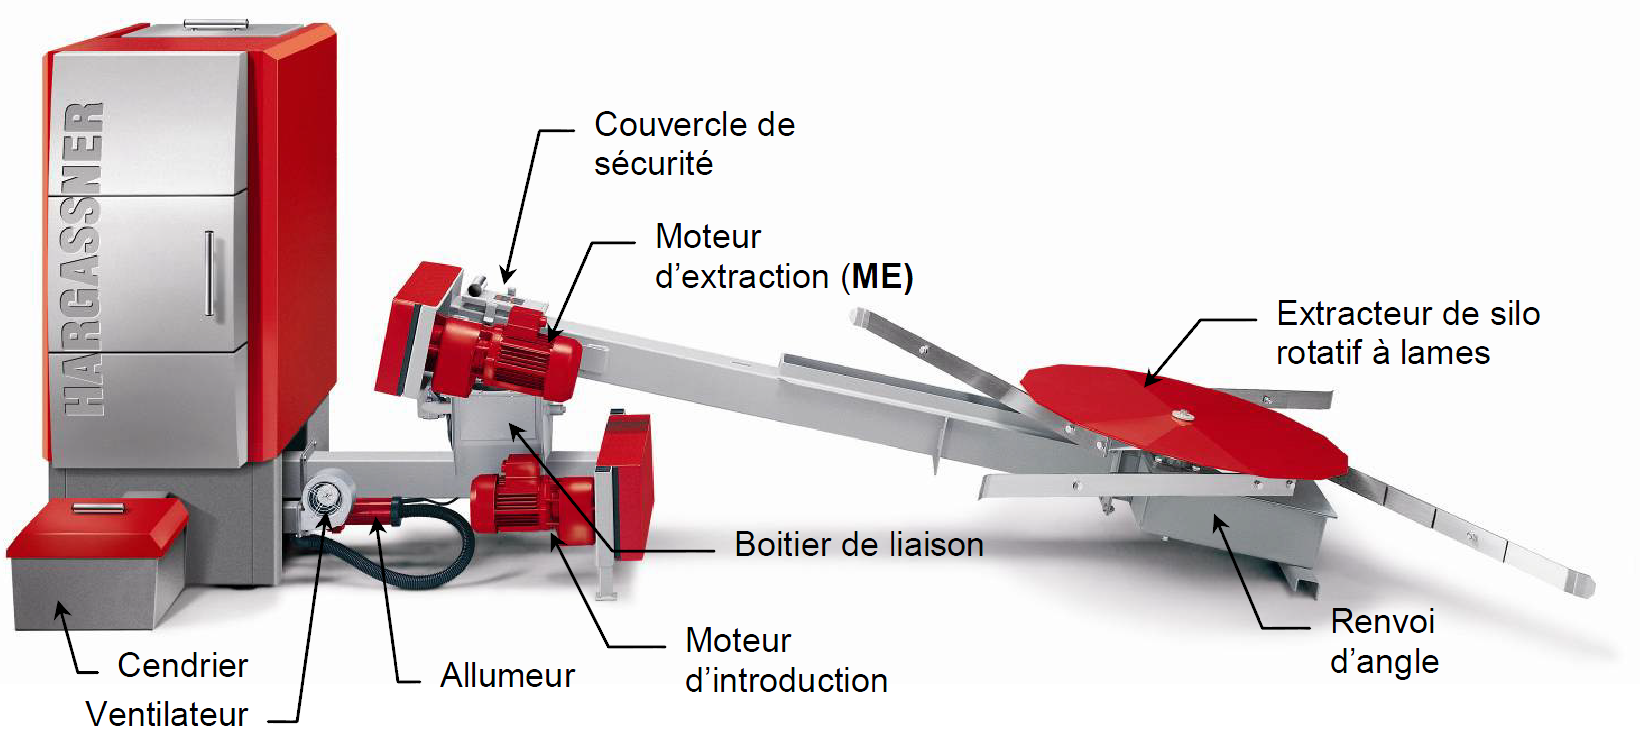
\includegraphics[width=\linewidth]{img/Fig1.png}
\caption{Chaudière}
\label{fig:image9}
\end{center}
\end{minipage}
\hfill
\begin{minipage}[c]{.6\linewidth}
Dans le cadre du \og Grenelle de l'environnement \fg et de la mise en place de la \og taxe carbone \fg, l'avenir du chauffage est conditionné au fait que la biomasse est neutre en dégagement de CO2. HARGASSNER développe la technologie du chauffage au bois déchiqueté et aux granulés de bois dans le but de concilier un chauffage à la fois écologique et confortable d'utilisation. L'étude porte sur la chaudière HSV 30, alimentée en bois déchiqueté, qui développe une puissance de chauffe de 25 à 35 kW.
\end{minipage}
\end{figure}

\begin{figure}[htbp]
\begin{minipage}[c]{.35\linewidth}
Le bois déchiqueté est amené jusqu'à la chaudière dans un premier temps à l'aide d'un extracteur à lames puis de la vis d'extraction et enfin par la vis d'introduction. Il est alors brûlé au sein d'un foyer réfractaire développant des gaz dans la chambre de combustion. Les gaz sont dépoussiérés dans la chambre de détente avant de passer dans un échangeur tubulaire équipé de turbulateurs. 
\end{minipage}
\hfill
\begin{minipage}[c]{.6\linewidth}
\begin{center}
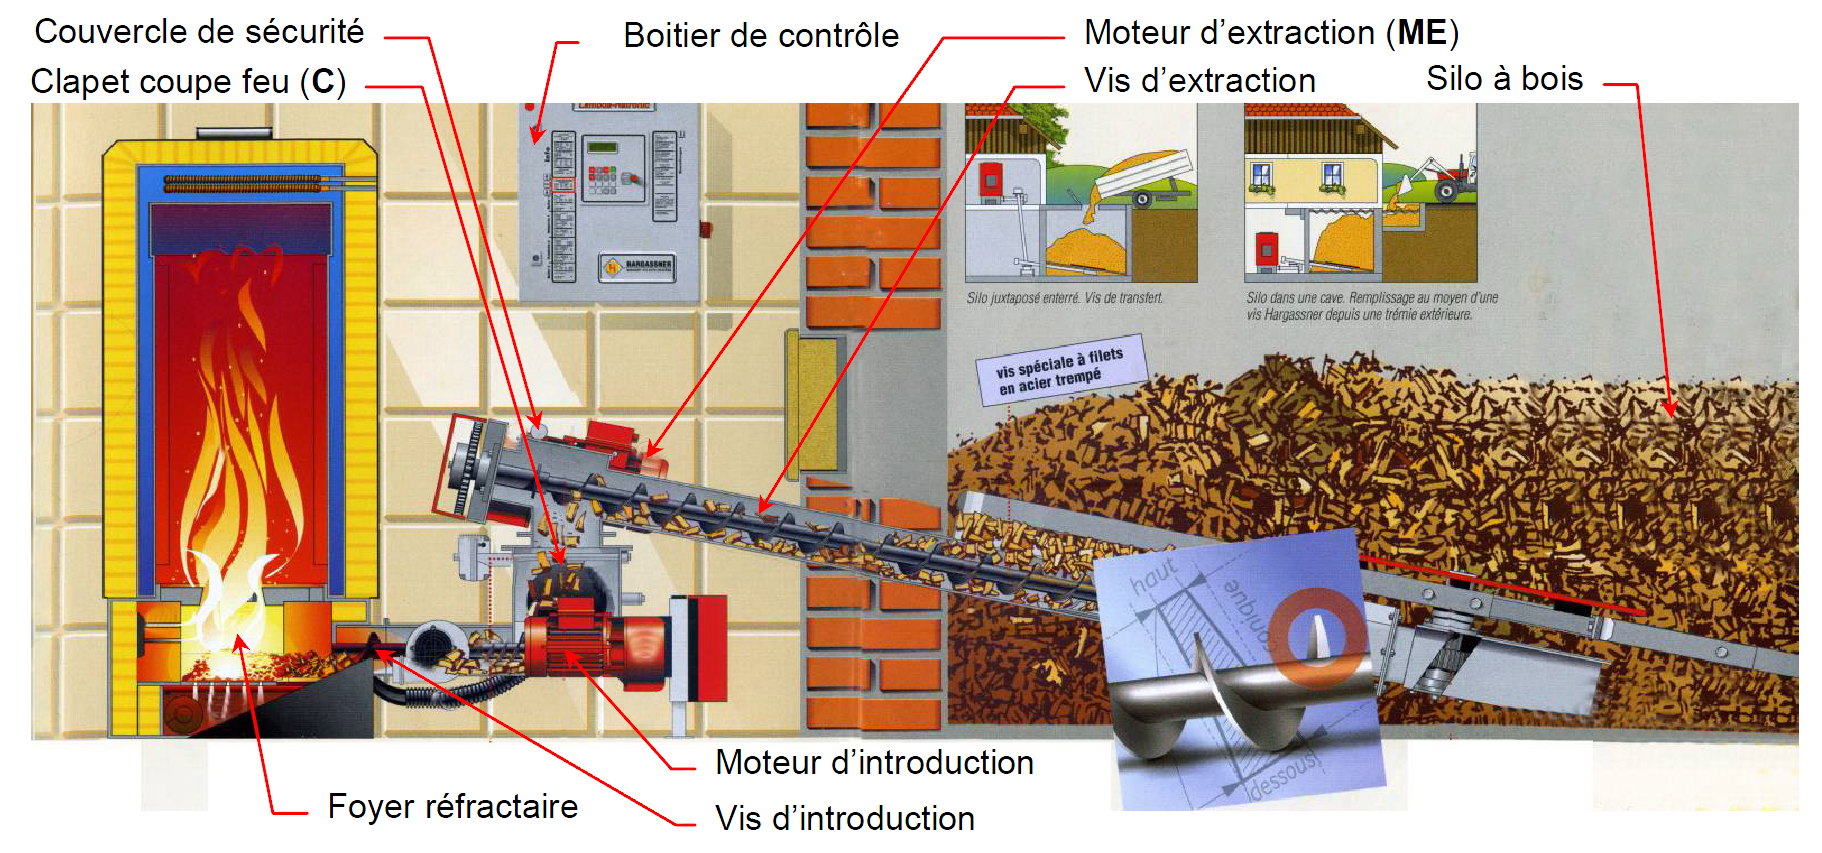
\includegraphics[width=\linewidth]{img/Fig2.png}
\caption{Fonctionnement}
\label{fig:image10}
\end{center}
\end{minipage}
\end{figure}

Ces turbulateurs augmentent l'efficacité de l'échangeur et permettent son nettoyage automatique. L'échangeur permet le chauffage de l'eau à partir des fumées. Une vis de dépoussiérage et une vis de décendrage, associées aux turbulateurs évacuent automatiquement les cendres et les suies dans un cendrier.

\subsection{Etude du point de vue des mouvements}

Le but de cette partie est d'étudier la relation entre la vitesse de rotation du moteur de décendrage (MD) et la vitesse de translation des turbulateurs. En effet cette vitesse est un élément déterminant pour un nettoyage optimum de l'échangeur qui contribue au bon rendement de la chaudière.
Le cahier des charges stipule que la vitesse maximum des turbulateurs par rapport à l'échangeur soit comprise entre 0,15 m/s et 0,25 m/s.

Dans cette partie, l'étudier va porter sur la relation entre la rotation du moteur et le mouvement de la tringle de commande 4.

On considère le mécanisme plan (dans le plan ($\overrightarrow{x_0}$,$\overrightarrow{y_0}$)), dans la situation proposée sur le schéma cinématique de la figure \ref{fig:image11}, à l'échelle 1/3, et dans le repère $R_0$(O,$\overrightarrow{x_0}$,$\overrightarrow{y_0}$,$\overrightarrow{z_0}$) .

\begin{itemize}
	\item La manivelle d'entrainement 1 est mise en rotation par le motoréducteur de décendrage (MD), lié au bâti 0, à partir d'une liaison pivot d'axe O,$\overrightarrow{z}$ à la vitesse de rotation $\omega_{10}.\overrightarrow{z}$, tel que l'angle $\theta_{10}=(\overrightarrow{x_0}$,$\overrightarrow{x_1}$) et $\overrightarrow{OA}=r.\overrightarrow{x_1}$,
	\item Le repère $R_1$(O,$\overrightarrow{x_1}$,$\overrightarrow{y_1}$,$\overrightarrow{z}$) est lié à la manivelle d'entrainement 1,
	\item La bielle 2 est liée à la manivelle d'entrainement 1 par une liaison pivot d'axe A,$\overrightarrow{z}$,
	\item Le repère $R_2$(A,$\overrightarrow{x_2}$,$\overrightarrow{y_2}$,$\overrightarrow{z}$) est lié à la bielle 2. On note l'angle $\theta_{20}=(\overrightarrow{x_0}$,$\overrightarrow{x_2}$),
	\item L'accouplement 3 est lié à la bielle 2 par une liaison pivot d'axe B,$\overrightarrow{z}$,
	\item Le repère $R_3$(B,$\overrightarrow{x_3}$,$\overrightarrow{y_3}$,$\overrightarrow{z}$) est lié à l'accouplement 3. On note $\overrightarrow{AB}=l.\overrightarrow{y_2}$,
	\item L'accouplement 3 est lié au bâti 0 par une liaison pivot d'axe C,$\overrightarrow{z}$,
	\item On note l'angle $\theta_{30}=(\overrightarrow{x_0}$,$\overrightarrow{x_3}$) et $\overrightarrow{BC}=-R.\overrightarrow{x_3}$,
	\item On note $\overrightarrow{CO}=L.\overrightarrow{x_0}$.
\end{itemize}

\begin{figure}[htbp]
\begin{center}
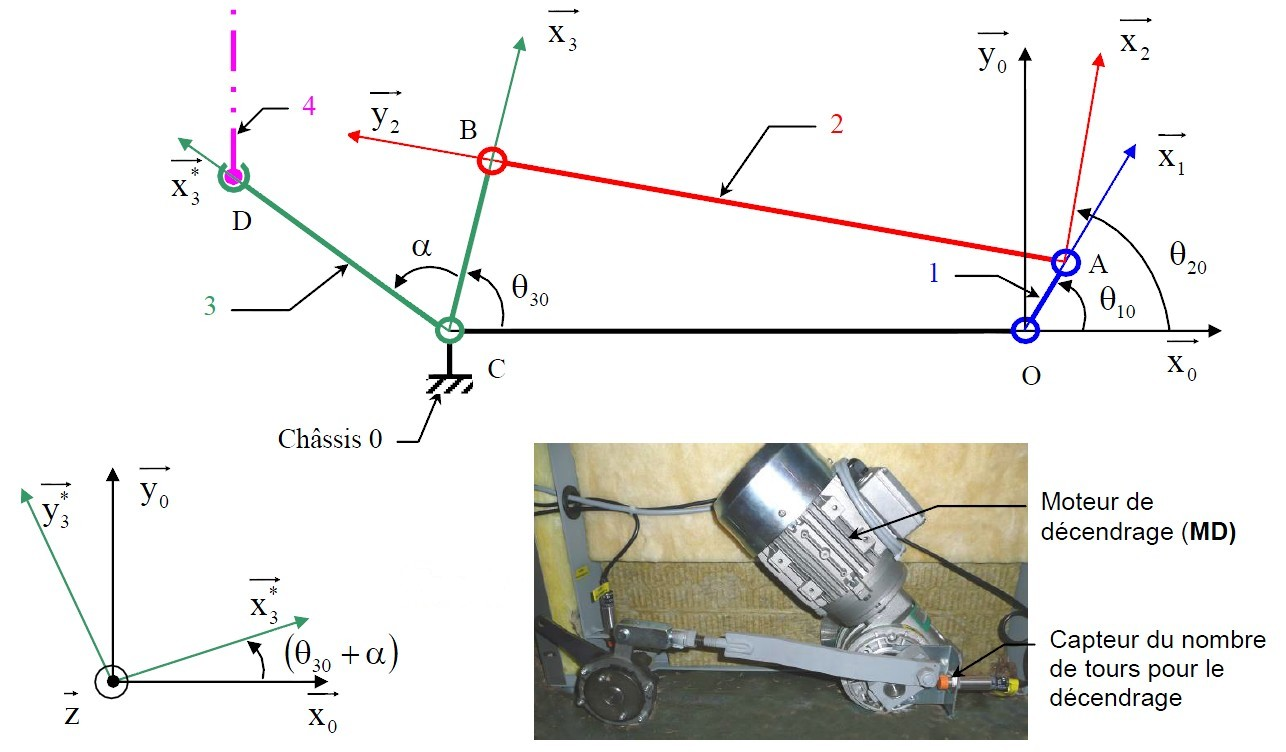
\includegraphics[width=0.7\linewidth]{img/Chaudiere_cin.jpg}
\caption{Schéma cinématique}
\label{fig:image11}
\end{center}
\end{figure}


\paragraph{Question 1:}
Écrire la fermeture géométrique pour les centres de liaison O, A, B et C.
En déduire une relation entre $\theta_{30}$ et $\theta_{10}$ uniquement en fonction de r, R, L et l . Cette relation permettrait d'obtenir $\theta_{30}$ en fonction de $\theta_{10}$.

\paragraph{Question 2:}

Quelle méthode faudrait-il appliquer pour en déduire la relation entre la vitesse
de rotation $\omega_{10}$ de la manivelle 1 par rapport au bâti 0, et la vitesse de rotation $\omega_{30}$ de l'accouplement 3 par rapport au bâti 0 (il n'est pas demandé de calcul).

~\

L'accouplement 3 est formé de deux bras décalés l'un de l'autre d'un angle $\alpha=(\overrightarrow{x_3},\overrightarrow{x_3^*})$ comme le montre la figure \ref{fig:image11}. La tringle de commande 4 est en liaison pivot d'axe D,$\overrightarrow{z}$ avec l'accouplement 3 au point D et tel que $\overrightarrow{CD}=d.\overrightarrow{x_3^*}$.

\paragraph{Question 3:}

Ecrire les torseurs suivants $\left\{V_{O\in 1/0}\right\}$, $\left\{V_{A\in 2/1}\right\}$, $\left\{V_{B\in 3/2}\right\}$, $\left\{V_{C\in 3/0}\right\}$.

Déplacer tous ces torseurs au point C.

Ecrire la chaîne torsorielle suivante: $\left\{V_{C\in 1/0}\right\}+\left\{V_{C\in 2/1}\right\}+\left\{V_{C\in 3/2}\right\}=\left\{V_{C\in 3/0}\right\}$, afin de déterminer toutes les composantes de $\left\{V_{C\in 3/0}\right\}$ en fonction des paramètres géométriques du systèmes, de $\theta_{10}$ et de $\omega_{10}$.

Déplacer le torseur $\left\{V_{C\in 3/0}\right\}$ au point D, afin de déterminer $\overrightarrow{V_{D\in 3/0}}$ en fonction des paramètres géométriques du systèmes, de $\theta_{10}$ et de $\omega_{10}$.

\newpage

\section{Plate-forme d'exploration tout terrain}

\begin{figure}[htbp]
\begin{minipage}[c]{.35\linewidth}
\begin{center}
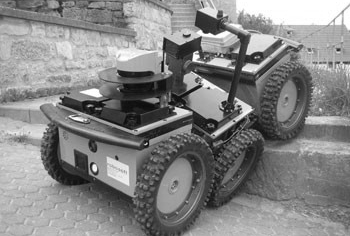
\includegraphics[width=\linewidth]{img/Robot1.png}
\caption{Robot d'exploration}
\label{fig:image12}
\end{center}
\end{minipage}
\hfill
\begin{minipage}[c]{.6\linewidth}
Le robuROC 6, figure \ref{fig:image12} est un robot mobile développé par la société ROBOSOFT. Cette plate-forme robotisée a été conçue pour des applications de recherche et d'exploration en milieu extérieur.
\end{minipage}
\end{figure}

\begin{figure}[htbp]
\begin{minipage}[c]{.4\linewidth}
Elle est équipée de 6 roues motrices indépendantes, de même diamètre, montées par paires sur 3 podes articulés en tangage et en roulis \ref{fig:image13}. La cinématique permet à la plate-forme de se conformer au relief parcouru et de franchir des obstacles du type trottoirs, escaliers. Le robuROC 6 a été conçu pour se déplacer en zones urbaines et peut aussi s'adapter à tous types de milieux.  
\end{minipage}
\hfill
\begin{minipage}[c]{.55\linewidth}
\begin{center}
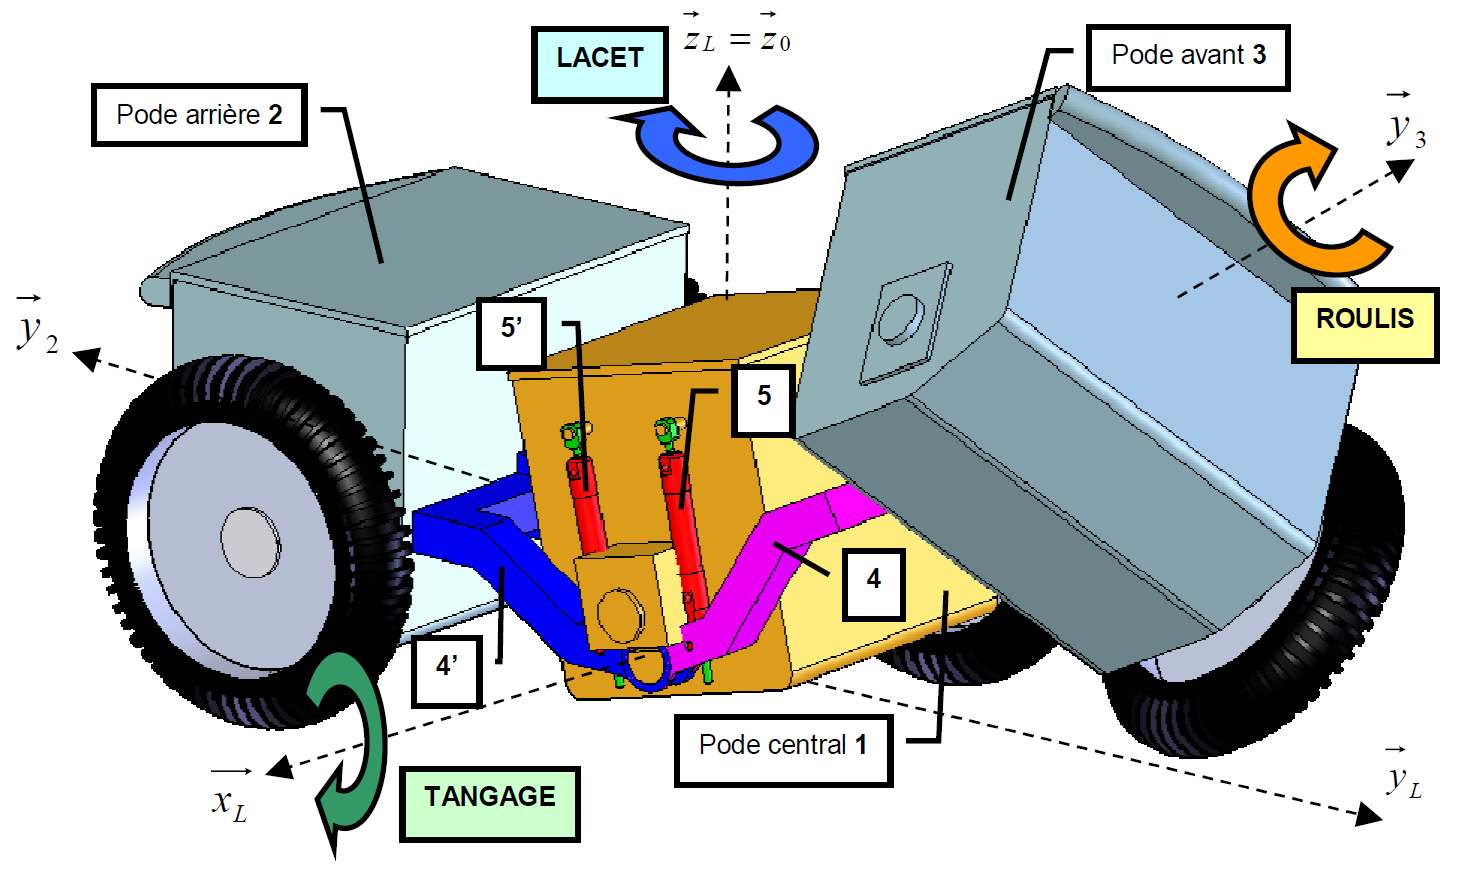
\includegraphics[width=\linewidth]{img/Robot_cin.png}
\caption{Schéma cinématique robot}
\label{fig:image13}
\end{center}
\end{minipage}
\end{figure}

La plate-forme peut se déplacer, sous conditions, en mode 6 roues ou 4 roues pour certaines applications particulières, comme le montre la figure \ref{fig:image14}.

\begin{figure}[htbp]
\begin{minipage}[c]{.32\linewidth}
\begin{center}
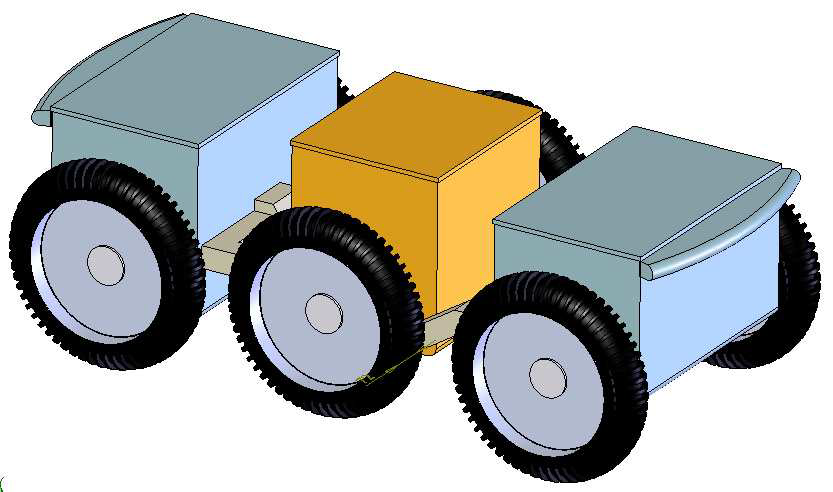
\includegraphics[width=\linewidth]{img/Robot2.png}
Mode 6 roues
\end{center}
\end{minipage}
\hfill
\begin{minipage}[c]{.32\linewidth}
\begin{center}
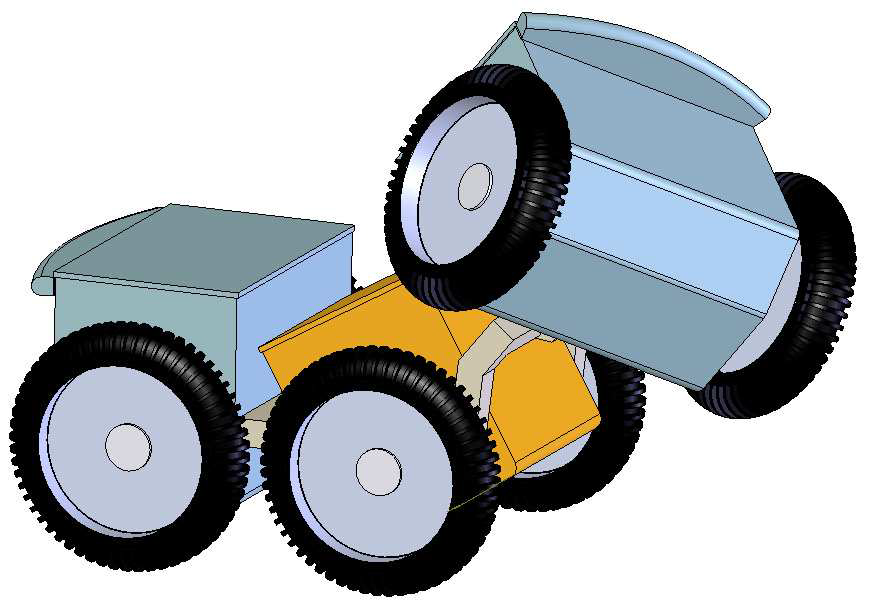
\includegraphics[width=\linewidth]{img/Robot3.png}
Mode 4 roues Déplacement
\end{center}
\end{minipage}
\hfill
\begin{minipage}[c]{.32\linewidth}
\begin{center}
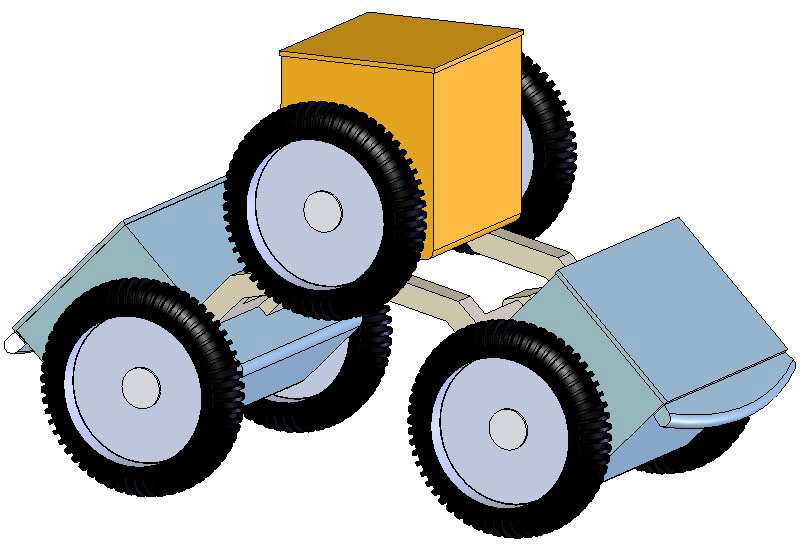
\includegraphics[width=\linewidth]{img/Robot4.png}
Mode 4 roues Observation
\end{center}
\end{minipage}
\caption{Modes de déplacement}
\label{fig:image14}
\end{figure}

Les trois podes sont articulés en tangage et en roulis, figure \ref{fig:image13}. Le mouvement de tangage est guidé par deux liaisons pivot (d'axe de direction $\overrightarrow{x_1}$), respectivement entre le bras d'articulation avant 4 et le pode central 1 et entre le bras d'articulation arrière 4' et le pode central 1. Le système hydraulique de suspension permet l'amortissement (mode passif) et la motorisation de ce mouvement (mode actif). Les vérins 5 (côté droit) et 6 (côté gauche) sont en liaison avec le bras d'articulation avant 4 et le pode central 1. Les vérins 5' (côté droit) et 6' (côté gauche) sont en liaison avec le bras d'articulation arrière 4' et le pode central 1. Le mouvement de roulis est assuré par deux liaisons pivot entre le pode avant 3 et le bras d'articulation avant 4 (liaison d'axe de direction $\overrightarrow{y_3}$) d'une part, et entre le pode arrière 2 et le bras d'articulation arrière 4' (liaison d'axe de direction $\overrightarrow{y_2}$) d'autre part. Ce mouvement n'est pas motorisé. 

L'ensemble E={bras d'articulation avant 4 + pode avant 3 + roues avant} est soulevé par les vérins avant 5 et 6 placés de part et d'autre du pode central 1. Le modèle cinématique retenu est défini sur la figure \ref{fig:image145}. Le mécanisme est constitué :
\begin{itemize}
	\item du pode central fixe 1 : repère associé $R_1=(O_1,\overrightarrow{x_1},\overrightarrow{y_1},\overrightarrow{z_1})$,
	\item de l'ensemble E={bras d'articulation avant 4 + pode avant 3 + roues avant} : repère associé $R_1=(O_1,\overrightarrow{x_1},\overrightarrow{y_3},\overrightarrow{z_3})$ avec $\beta=(\overrightarrow{y_1},\overrightarrow{y_3})=(\overrightarrow{z_1},\overrightarrow{z_3})$,
	\item du vérin 5 constitué du corps $5_1$ et de la tige $5_2$ : repère associé $R_5=(A,\overrightarrow{x_1},\overrightarrow{y_5},\overrightarrow{z_5})$ avec $\gamma=(\overrightarrow{y_3},\overrightarrow{y_5})=(\overrightarrow{z_3},\overrightarrow{z_5})$,
	\item du vérin 6 non représenté car ayant le même comportement que le vérin 5,
	\item Paramétrage : $\overrightarrow{O_1A}=d_4.\overrightarrow{y_3}$, $\overrightarrow{AB}=\lambda.\overrightarrow{y_5}$, $\overrightarrow{O_1B}=d_1.\overrightarrow{y_1}+h_1.\overrightarrow{z_1}$, la vitesse de rentrée/sortie du vérin sera appelée $V$,
	\item Valeurs numériques : $d_4=70mm$, $h_1=292mm$, $d_1=76mm$, $\beta \in \left[-45 \degrees , +30 \degrees\right]$.
\end{itemize}

\begin{figure}[htbp]
\begin{minipage}[c]{.48\linewidth}
\begin{center}
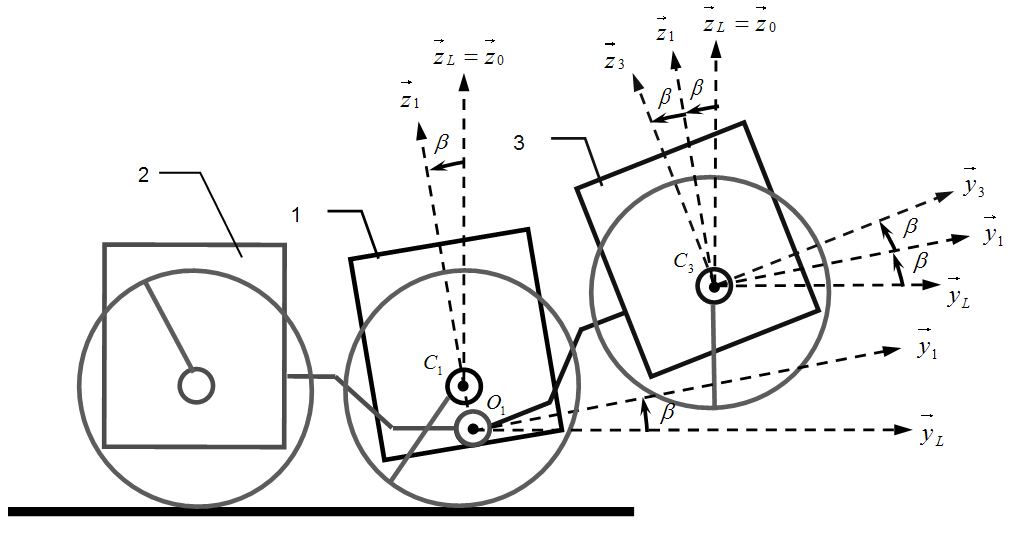
\includegraphics[width=\linewidth]{img/Robot-cin1.png}
\end{center}
\end{minipage}
\hfill
\begin{minipage}[c]{.48\linewidth}
\begin{center}
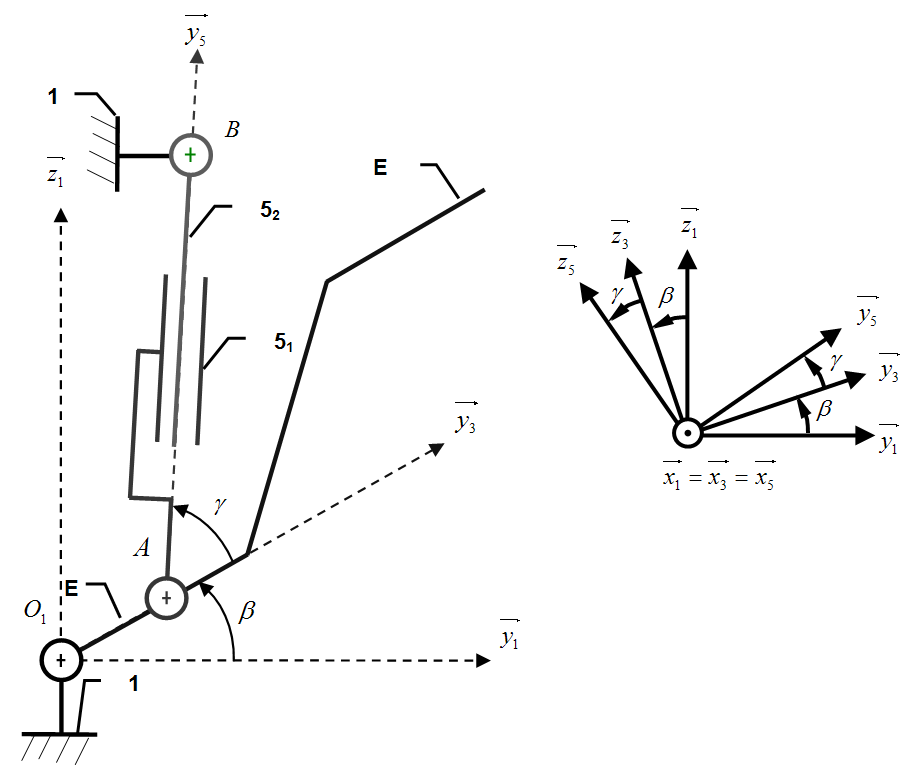
\includegraphics[width=\linewidth]{img/Robot-cin2.png}
\end{center}
\end{minipage}
\caption{Schémas cinématiques}
\label{fig:image145}
\end{figure}

\paragraph{Question 1:}

Exprimer $\lambda$ en fonction de $d_4$, $h_1$, $d_1$ et $\beta$.

Calculer les valeurs numériques d'élongation minimale $\lambda_{min}$, maximale $\lambda_{max}$ ainsi que la course du vérin 5.

\paragraph{Question 2:}

Ecrire les torseurs suivants, $\left\{V_{O_1\in E/1}\right\}$, $\left\{V_{A\in 5_1/E}\right\}$, $\left\{V_{A\in 5_2/5_1}\right\}$, $\left\{V_{B\in 5_2/1}\right\}$.

Déplacer tous ces torseurs au point A.

Ecrire la chaîne torsorielle suivante, $\left\{V_{A\in E/1}\right\}+\left\{V_{A\in 5_1/E}\right\}+\left\{V_{A\in 5_2/5_1}\right\}=\left\{V_{B\in 5_2/1}\right\}$ afin de déterminer toutes les composantes de $\left\{V_{O_1\in E/1}\right\}$ en fonction des paramètres géométriques du systèmes, de $\beta$ et de la vitesse $V$ de déplacement du vérin.

Déterminer alors la vitesse de rotation $\omega{E/1}$ en fonction des paramètres géométriques du systèmes, de $\beta$ et de la vitesse $V$ de déplacement du vérin.

\newpage

\section{Presse multi poinçonnage}

\begin{figure}[htbp]
\begin{minipage}[c]{.65\linewidth}
Un moteur asynchrone assure la rotation d'un dispositif \og vilebrequin + coulisseau \fg qui entraîne les outils en translation. Un codeur situé sur l'arbre moteur permet de connaître la position du vilebrequin.

Le mouvement du coulisseau est symbolisé par le diagramme suivant, figure \ref{fig:image15}, $\theta$ représente la position du vilebrequin.
\end{minipage}
\hfill
\begin{minipage}[c]{.3\linewidth}
\begin{center}
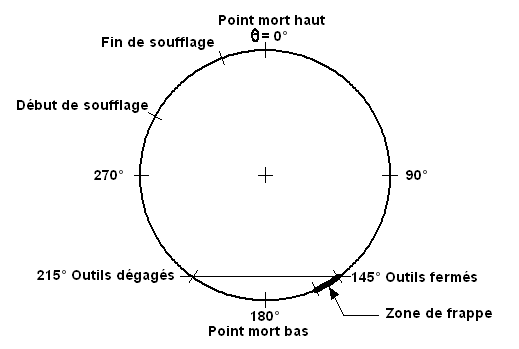
\includegraphics[width=\linewidth]{img/Poinc1.png}
\caption{Mouvement du coulisseau}
\label{fig:image15}
\end{center}
\end{minipage}
\end{figure}

\begin{figure}[htbp]
\begin{minipage}[c]{.3\linewidth}
\begin{center}
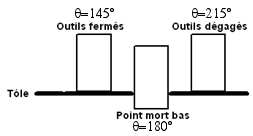
\includegraphics[width=\linewidth]{img/Poinc2.png}
\caption{Mouvement du poinçon}
\label{fig:image16}
\end{center}
\end{minipage}
\hfill
\begin{minipage}[c]{.65\linewidth}
Lorsque le coulisseau est suffisamment remonté, les tôles sont acheminées d'un pas par un système de pince. La pince est entraînée en translation par un moteur à courant continu avant le poinçonnage suivant. Après le poinçonnage les outils remontent, les couvercles
restent accrochés aux outils, un dispositif de soufflage permet de les décrocher, comme le montre la figure \ref{fig:image16}.
\end{minipage}
\end{figure}

\begin{figure}[htbp]
\begin{minipage}[c]{.45\linewidth}
On considère, figure \ref{fig:image16}, une partie de la presse composée d'un bâti (S0), d'un vilebrequin (S1), d'une bielle (S2) et d'un coulisseau (S3). Le vilebrequin est entraîné par un moteur et un dispositif \og poulies-courroie \fg de rapport de réduction $\frac{1}{4}$(non représenté ici). Un système de compensation (2 vérins) annule le poids du coulisseau.
\end{minipage}
\hfill
\begin{minipage}[c]{.5\linewidth}
\begin{center}
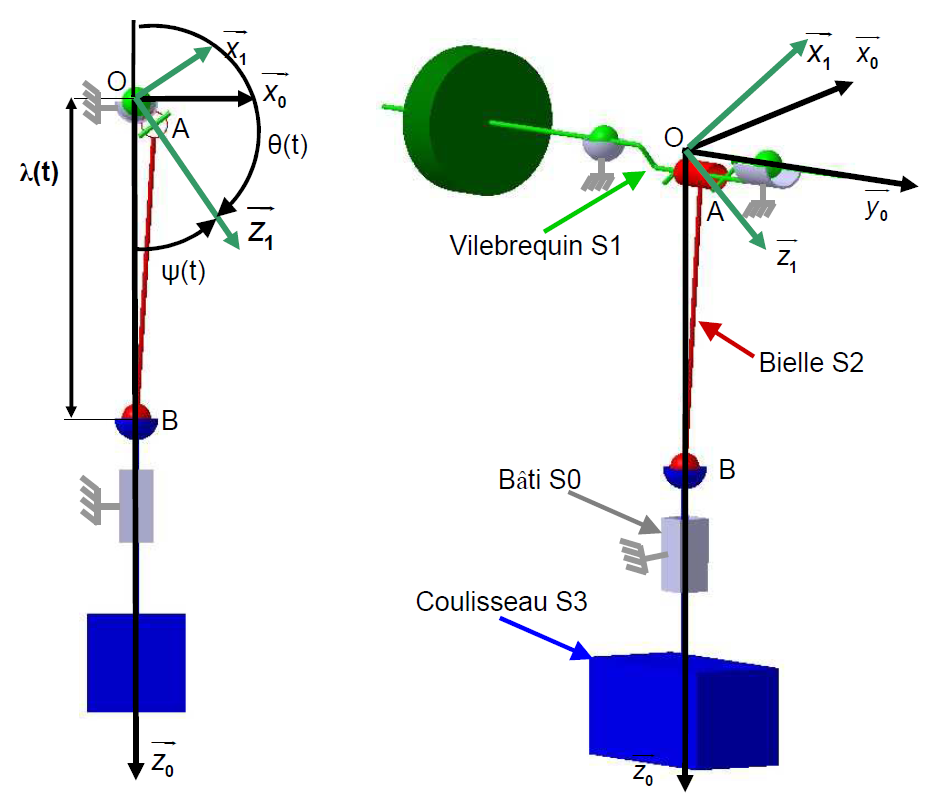
\includegraphics[width=\linewidth]{img/Poinc_cin2.png}
\caption{Schéma cinématique}
\label{fig:image16}
\end{center}
\end{minipage}
\end{figure}


Soit $R_0(B,\overrightarrow{x_0},\overrightarrow{y_0},\overrightarrow{z_0})$ un repère lié à (S0) (fixe). Le solide (S1) est en liaison pivot d'axe $(O,\overrightarrow{y_0})$ par rapport au solide (S0). $R_1(A,\overrightarrow{x_1},\overrightarrow{y_1},\overrightarrow{z_1})$ est un repère lié à (S1). Posons $\gamma=(\overrightarrow{z_0},\overrightarrow{z_1})$ avec $\dot{\gamma(t)}=\omega_v(t)$ avec $\omega_v$ constante positive exprimée en radians par seconde. On pose $\overrightarrow{OA}=a.\overrightarrow{z_1}$ avec A centre de la liaison entre (S1) et (S2). a = 60 mm.

Le solide (S2) est en liaison pivot d'axe (A,$\overrightarrow{y_0}$) par rapport à (S1). $R_2(A,\overrightarrow{x_2},\overrightarrow{y_2},\overrightarrow{z_2})$ est un repère lié à (S2). On pose $\beta=(\overrightarrow{z_0},\overrightarrow{z_2})$. Soit B le centre de la liaison entre (S2) et (S0) tel que : $\overrightarrow{AB}=b.\overrightarrow{z_2}$. b = 600 mm.
Enfin, il y a une liaison glissière entre le solide (S0) et (S3) telle que $\overrightarrow{OB}=\lambda.\overrightarrow{z_0}$.

\paragraph{Question 1:}

Par une fermeture géométrique trouver la relation entre $\lambda$ et $\gamma$.

\begin{figure}[htbp]
\begin{minipage}[c]{.6\linewidth}
\begin{center}
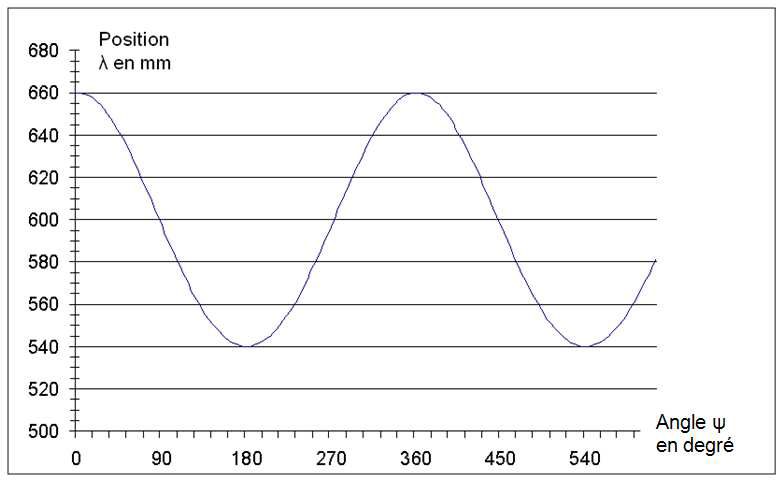
\includegraphics[width=\linewidth]{img/Poinc3.png}
\caption{Loi entrée/sortie}
\label{fig:image17}
\end{center}
\end{minipage}
\hfill
\begin{minipage}[c]{.45\linewidth}
\begin{center}
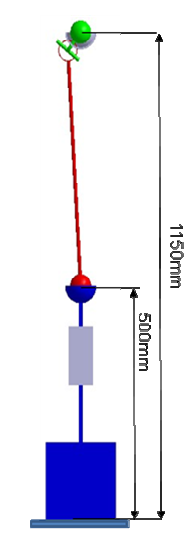
\includegraphics[width=0.3\linewidth]{img/Poinc4.png}
\caption{Schéma plan}
\label{fig:image18}
\end{center}
\end{minipage}
\end{figure}

La figure \ref{fig:image17} représente la loi entrée/sortie $\lambda$ en fonction de $\gamma$ que vous venez de déterminer et la 
figure \ref{fig:image18} représente la position de la presse au moment de la frappe.

\paragraph{Question 2:}

En déduire $\lambda$ et $\gamma$ au moment de la frappe.

On peut exprimer $\lambda$ sous la forme: $\lambda=a.cos(\gamma)+\sqrt{b^2-a^2.sin^2(\gamma)}$

On considèrera les deux liaisons entre $S_1$ et $S_0$ comme une seule liaison pivot.

\begin{figure}[htbp]
\begin{minipage}[c]{.55\linewidth}
\paragraph{Question 3:}

Ecrire les torseurs suivants, $\left\{V_{O\in S_1/S_0}\right\}$, $\left\{V_{A\in S_2/S_1}\right\}$, $\left\{V_{B\in S_3/S_2}\right\}$, $\left\{V_{B\in S_3/S_0}\right\}$.

Déplacer tous ces torseurs au point B.

Ecrire la chaîne torsorielle suivante, $\left\{V_{B\in S_1/S_0}\right\}+\left\{V_{B\in S_2/S_1}\right\}+\left\{V_{B\in S_3/S_2}\right\}=\left\{V_{B\in S_3/S_0}\right\}$ afin de déterminer toutes les composantes de $\left\{V_{B\in S_3/S_0}\right\}$ en fonction des paramètres géométriques du systèmes, de $\gamma(t)$ et de la vitesse $\omega_v(t)$.

Déterminer alors la vitesse de rotation $\overrightarrow{V_{B \in S_3/S_0}}$ en fonction des paramètres géométriques du systèmes, de $\gamma(t)$ et de la vitesse $\omega_v(t)$.
\end{minipage}
\hfill
\begin{minipage}[c]{.4\linewidth}
\begin{center}
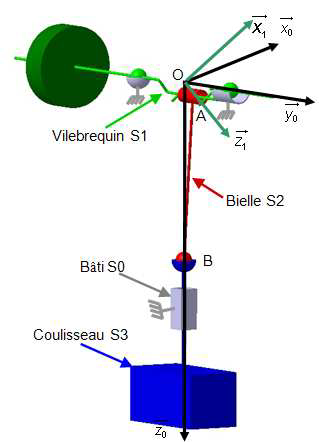
\includegraphics[width=\linewidth]{img/Poinc_cin.png}
\caption{Schéma cinématique}
\label{fig:image19}
\end{center}
\end{minipage}
\end{figure}

\end{document}
